% Quantum kernel classification as one picture (notebook 45d, Section 1).
% Top row (quantum device): two data points x, x' -> overlap (inversion) circuit U(x) then U^dagger(x') on |0>^N ->
%   measure all qubits -> the frequency of 0...0 estimates k(x,x') = |<phi(x')|phi(x)>|^2.
% Bottom row (classical computer): data set of two concentric rings -> kernel matrix K_ij for all training pairs ->
%   SVM dual problem (convex quadratic programme) -> decision function f(x) = sum_i alpha_i y_i k(x_i,x) + b,
%   whose zero level is the circular decision boundary.
\documentclass[tikz,border=6pt]{standalone}
\usepackage{amsmath,amssymb,bm}
\usetikzlibrary{arrows.meta,positioning,calc,fit,decorations.pathreplacing}
\newcommand{\ket}[1]{\lvert #1\rangle}
\begin{document}
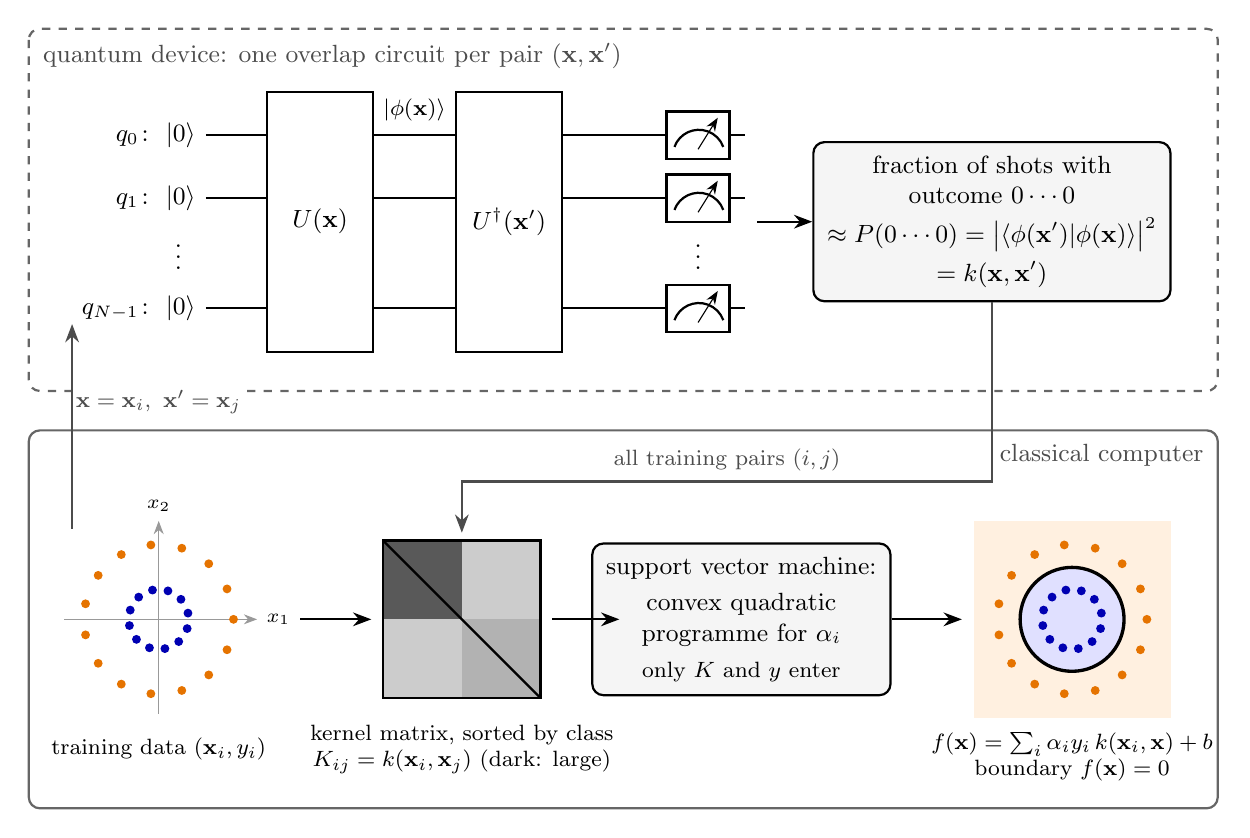
\begin{tikzpicture}[thick, >=Stealth, font=\small,
    gate/.style={draw, fill=white, minimum height=3.3cm, minimum width=1.35cm, inner sep=2pt},
    box/.style={draw, rounded corners, fill=black!4, align=center, inner sep=5pt}]
  % ================================================================ quantum device (top)
  \draw[dashed, rounded corners, black!60] (-0.5,1.35) rectangle (14.6,-3.25);
  \node[anchor=north west, black!70] at (-0.45,1.3) {quantum device: one overlap circuit per pair $(\mathbf x,\mathbf x')$};
  \foreach \y/\lab in {0/{q_0}, -0.8/{q_1}, -2.2/{q_{N-1}}} {
    \node[anchor=east] at (1.75,\y) {$\lab\colon\ \ket{0}$};
    \draw (1.75,\y) -- (8.6,\y);
  }
  \node at (1.4,-1.45) {$\vdots$};
  \node[gate] at (3.2,-1.1) {$U(\mathbf x)$};
  \node[gate] at (5.6,-1.1) {$U^\dagger(\mathbf x')$};
  \node[above, font=\footnotesize] at (4.4,0.05) {$\ket{\phi(\mathbf x)}$};
  \foreach \y in {0,-0.8,-2.2} {
    \draw[fill=white] (7.6,\y+0.3) rectangle (8.4,\y-0.3);
    \draw (7.7,\y-0.15) arc (160:20:0.33);
    \draw[->, thin] (8.0,\y-0.18) -- (8.25,\y+0.22);
  }
  \node at (8.0,-1.45) {$\vdots$};
  \draw[->] (8.75,-1.1) -- (9.45,-1.1);
  \node[box, anchor=west] (kx) at (9.45,-1.1) {fraction of shots with\\ outcome $0\cdots0$\\[3pt]
     $\approx P(0\cdots0)=\big\vert\langle\phi(\mathbf x')\vert\phi(\mathbf x)\rangle\big\vert^2$\\[3pt]
     $=k(\mathbf x,\mathbf x')$};
  % ================================================================ classical computer (bottom)
  \draw[rounded corners, black!60] (-0.5,-3.75) rectangle (14.6,-8.55);
  \node[anchor=north east, black!70] at (14.55,-3.8) {classical computer};
  % data: two rings
  \begin{scope}[shift={(1.15,-6.15)}]
    \draw[black!40, thin, ->] (-1.2,0) -- (1.25,0) node[right, font=\scriptsize, black] {$x_1$};
    \draw[black!40, thin, ->] (0,-1.2) -- (0,1.25) node[above, font=\scriptsize, black] {$x_2$};
    \foreach \a in {0,30,...,330} \fill[blue!70!black] ({0.38*cos(\a+12)},{0.38*sin(\a+12)}) circle (1.6pt);
    \foreach \a in {0,24,...,336} \fill[orange!90!black] ({0.95*cos(\a)},{0.95*sin(\a)}) circle (1.6pt);
    \node[font=\footnotesize, align=center] at (0,-1.65) {training data $(\mathbf x_i,y_i)$};
  \end{scope}
  % kernel matrix
  \begin{scope}[shift={(4.0,-5.15)}]
    \fill[black!65] (0,0) rectangle (1,-1);
    \fill[black!20] (1,0) rectangle (2,-1);
    \fill[black!20] (0,-1) rectangle (1,-2);
    \fill[black!30] (1,-1) rectangle (2,-2);
    \draw (0,0) rectangle (2,-2);
    \draw[black, thick] (0,0) -- (2,-2);
    \node[font=\footnotesize, align=center] at (1,-2.65) {kernel matrix, sorted by class\\ $K_{ij}=k(\mathbf x_i,\mathbf x_j)$ (dark: large)};
  \end{scope}
  % SVM box
  \node[box] (svm) at (8.55,-6.15) {support vector machine:\\[2pt] convex quadratic\\ programme for $\alpha_i$\\[2pt]
     {\footnotesize only $K$ and $y$ enter}};
  % decision boundary
  \begin{scope}[shift={(12.75,-6.15)}]
    \fill[orange!12] (-1.25,-1.25) rectangle (1.25,1.25);
    \fill[blue!12] (0,0) circle (0.66);
    \draw[very thick] (0,0) circle (0.66);
    \foreach \a in {0,30,...,330} \fill[blue!70!black] ({0.38*cos(\a+12)},{0.38*sin(\a+12)}) circle (1.6pt);
    \foreach \a in {0,24,...,336} \fill[orange!90!black] ({0.95*cos(\a)},{0.95*sin(\a)}) circle (1.6pt);
    \node[font=\footnotesize, align=center] at (0,-1.75) {$f(\mathbf x)=\sum_i\alpha_iy_i\,k(\mathbf x_i,\mathbf x)+b$\\ boundary $f(\mathbf x)=0$};
  \end{scope}
  % arrows
  \draw[->] (2.95,-6.15) -- (3.85,-6.15);
  \draw[->] (6.15,-6.15) -- (7.0,-6.15);
  \draw[->] (svm.east) -- (11.35,-6.15);
  % link between device and kernel matrix
  \draw[->, black!70] (kx.south) |- node[pos=0.75, above, font=\footnotesize] {all training pairs $(i,j)$} (5.0,-4.4) -- (5.0,-5.05);
  \draw[->, black!70] (0.05,-5.0) -- (0.05,-2.4) node[pos=0.62, right, font=\footnotesize, fill=white, inner sep=1pt] {$\mathbf x=\mathbf x_i,\ \mathbf x'=\mathbf x_j$};
\end{tikzpicture}
\end{document}
